\documentclass[conference]{IEEEtran}
\IEEEoverridecommandlockouts
\usepackage{textcomp}
\usepackage{xcolor}
\def\BibTeX{{\rm B\kern-.05em{\sc i\kern-.025em b}\kern-.08em
    T\kern-.1667em\lower.7ex\hbox{E}\kern-.125emX}}
\usepackage{cite}
\usepackage{balance} % to use \balance command for balancing
\usepackage{algorithmic}
\usepackage{algorithm}
\usepackage{mathrsfs,amsthm}
\usepackage{textcomp} 
%\usepackage{siunitx}
\usepackage{lettrine}
\usepackage{dirtytalk}
\usepackage[letterpaper,left=.62in, right=.62in, top=0.75in, bottom=1.0in]{geometry}
%\usepackage[a4paper,left=1in, right=1.0in, top=1.0in, bottom=1.0in]{geometry}
\usepackage{pslatex}			% use for Times new roman 
%\usepackage{sectsty}			% To control section, subsection.... font size
\usepackage{latexsym}
\usepackage{subfig}
\usepackage{graphicx}
\usepackage{caption}
\usepackage{subcaption}
\usepackage{float}

\usepackage{lipsum}
\usepackage{adjustbox}
\usepackage{longtable}
\usepackage{ltablex}
\usepackage{multirow}
\usepackage{tabularx}
\usepackage{array}
\usepackage{multicol}
\def\NoNumber#1{{\def\alglinenumber##1{}\State #1}\addtocounter{ALG@line}{-1}}


\usepackage{amssymb,amsmath,epsfig,latexsym,graphicx,bm,listings,color,amsthm,tabu}
\usepackage[utf8]{inputenc}

\usepackage{url}
\usepackage{comment}
%\ifCLASSOPTIONcompsoc
%    \usepackage[caption=false, font=normalsize, labelfont=sf, textfont=sf]{subfig}
%\else
%\usepackage[caption=false, font=footnotesize]{subfig}
%\fi

%\usepackage{epsfig}
\renewcommand\IEEEkeywordsname{Index Terms}
\begin{document}

\DeclareRobustCommand*{\IEEEauthorrefmark}[1]{%
  \raisebox{0pt}[0pt][0pt]{\textsuperscript{\footnotesize\ensuremath{#1}}}}

%\onecolumn

\title{A Contention Aware Connected Dominating Set Construction Algorithm for Wireless Ad-Hoc Networks}


\author{\IEEEauthorblockN{Chowdhury Nawrin Ferdous}
\IEEEauthorblockA{Department of Computer Science and Engineering\\
Bangladesh University of Engineering and Technology\\
Dhaka, Bangladesh\\
Email: bipashachowdhury03@gmail.com}
\and
\IEEEauthorblockN{Ashikur Rahman}
\IEEEauthorblockA{Department of Computer Science and Engineering\\
Bangladesh University of Engineering and Technology\\
Dhaka, Bangladesh\\
Email: ashikur@cse.buet.ac.bd}
}

%****************************
% The paper headers
%\markboth{Journal of \LaTeX\ Class Files,~Vol.~6, No.~1, January~2007}%
%{Shell \MakeLowercase{\textit{et al.}}: Bare Demo of IEEEtran.cls for Journals}
%*****************************

% make the title area
\maketitle

\begin{abstract}
%\label{abstract}
The nodes in wireless ad-hoc networks frequently need to broadcast messages for route discovery and other services. The naive flooding requires every node to forward a message exactly once and causes serious performance bottleneck due to redundant traffic, contention, and collision.One convenient solution to overcome this problem is to construct a connected dominating set (CDS) as virtual backbone. Several centralized and distributed algorithms have been designed to compute CDS in order to reduce the number of rebroadcasts. However, none of the approaches aim at minimizing contentions. Contention is a phenomenon that occurs when a group of nodes want to transmit over a shared channel. During contention only one node gets access to the channel and the others defer their transmission for a later time. In this paper, a new heuristic dubbed as \emph{Contention Aware Connected Dominating Set (CACDS)} has been proposed to construct a CDS that intelligently selects the nodes to reduce contention. A centralized algorithm has been deduced first to construct CDS using the global topology information.
Since it is difficult to gather the entire topology information, a distributed counterpart has also been presented where a node selects a subset of nodes from its immediate neighbors as forwarding nodes based on 2-hop neighborhood information and reduces contention. Experimental results show that proposed heuristics significantly reduce contention and outperform other state-of-the-art algorithms in minimizing contention with a little increase in number of forwarding nodes. 
\end{abstract}

\begin{IEEEkeywords}

 Contention, Wireless Ad-hoc Network, Connected Dominating Set.

\end{IEEEkeywords}
\IEEEpeerreviewmaketitle


\section{Introduction}
\label{introduction}
%\begin{introduction}
%\boldmath
A wireless ad-hoc network is a collection of several mobile nodes that dynamically form a network for communication without any pre-existing infrastructure or any centralized control. This network is popularly used in emergency search-and-rescue operations, decision making in the battlefield etc. where network needs to be deployed immediately but the base stations or fixed network or infrastructures are not available. The mobile nodes often cannot communicate with each other directly because of several causes such as limitation of power, improper utilization of channel and many more. So, they rely on several intermediate nodes (known as relays) to exchange data with one another over the network and thus the wireless multi-hop network is formed.
 %The mobility of the nodes causes continuous change in network topology which is the greatest concerns in wireless multi-hop network. 
 The nodes in these networks frequently need to broadcast messages for route discovery, periodic data dissemination, erasing an invalid route, locating a node,  or even for sending alarm signals in the entire network.
 
An effortless approach to perform broadcast is \emph{blind flooding}. Every node forwards a broadcast message exactly once in blind flooding. Though blind flooding ensures full coverage at high mobility but unfortunately, it results in redundant traffic, contention, and collision and finally leads to \textit{broadcast storm problem}\cite{tseng2002broadcast}. One solution to overcome these problems is to compute a virtual backbone based on the physical topology, and run any existing routing protocol over the virtual backbone\cite{butenko2004new}. 

The Connected Dominating Set (CDS) is a widely used approach in this context. A CDS is generally constructed by at first modeling the entire network as a graph $G$ where all nodes form a node set $V$ and the communication links between nodes form an edge set $E$. Then, a CDS of a graph $G$ contains a subset $D$ of the node set $V$ where any node in $D$ can reach any other node in $D$ by a path that stays entirely within $D$. That is, $D$ induces a connected sub-graph of $G$ and every node in $G$ either belongs to $D$ or is adjacent to a node in $D$.  Only the nodes belonging to CDS  participate in forwarding to convey the message in the entire network.

%hence they are known as the forwarding nodes of the network.
 A notable number of centralized and distributed algorithms ~\cite{yang2017routing, butenko2004new, luo2017new} have been devised to create CDS to reduce the number of packet forwarding. Although CDS based algorithms have been proposed to reduce redundancy, none of these works aim at minimizing contention. Contention means \textit{competition for resources}. The term is used especially in networks to describe the situation where two or more nodes attempt to transmit a message across the same medium at the same time. In a mobile ad-hoc network, after broadcasting a message by a mobile host, if more than one neighbors which are within their transmission range want to rebroadcast it, these transmissions may face serious contention with each other.
 
 The main contribution in this paper is to construct a connected dominating set in such a way so that the contention among the nodes in CDS is minimized. A couple of new heuristics have been proposed to construct the contention aware connected dominating set (CACDS) in this work. 
 
 A centralized algorithm has been deduced first to construct CDS using the global topology information of a wireless network. Since it is difficult to gather the entire topology information, a distributed version has also been presented where a node selects a subset of nodes from its immediate neighbors as forwarding nodes based on 2-hop neighborhood information. A demonstration of the efficiency of the distributed algorithm using the centralized algorithm as a benchmark is also provided in this work. Finally, a comprehensive simulation to analyze the behavior of the proposed algorithms and compare their performances with other state-of-the-art algorithms in terms of number of forwarding nodes and amount of contention has been presented. In centralized environment, with the increase of 0-5\% forwarding nodes, new heuristic generates almost 90-100\% contention free CDS and it increases the number of forwarding nodes by 1-5\% to mitigate almost 4-19\% contention in CDS in a distributed environment.

The rest of the paper is organized as follows. In Section 2, the basic idea of this work has been discussed. In Section 3, we present the state-of-the-art research works. Section 4 provides the important terminologies and considered state-of-art algorithms. Section 5 deals with the methodology of the new proposed algorithms with suitable examples. Section 6 demonstrates the simulation and performance evaluation and finally Section 7 concludes the paper highlighting the contribution, limitations  and possible future works.  
%\end{introduction}



\section{Basic Idea}
\label{Basic Idea}
Formally, a CDS of a graph $G$ is a set D of nodes with the following two properties:

(i) Any node in D can reach any other node in D using only the nodes that belong to D. 

(ii) Every node in G either belongs to D or is adjacent to a node in D. That is why D is called a dominating set of G.

Once the CDS is constructed broadcasting task is performed as follows:- if the source is in CDS then only the nodes in CDS need to forward the packet and the packet reaches all the nodes in the network because the nodes that are not in CDS must be neighbors of some node(s) in CDS. If the source is not in  CDS it can forward the packet to its neighbors and at least one of its neighbors is guaranteed to be in CDS. Thus the packet reaches one of the CDS nodes and all other nodes in CDS forward the packet like before.

 The main goal of this work is to construct a CDS 
 %in such a way so that when the nodes in CDS forward the message, the contentions among the nodes in CDS are as minimum as possible. In other word, a CDS will be constructed 
 that will intelligently select the nodes to reduce contention.  Upon receiving a packet from one node if two or more neighboring nodes try to rebroadcast the packet at the same time, there will occur contention. For example, consider the sample network of 7 nodes illustrated in Figure \ref{aa}.
 
\begin{figure}[h] 
    \centering
  \subfloat[]{%
       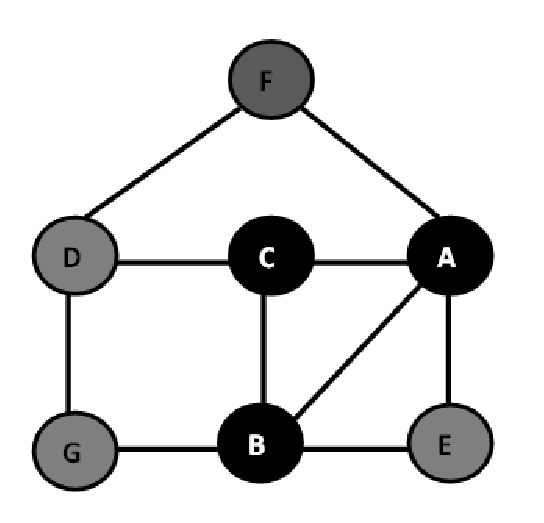
\includegraphics[width=0.5\linewidth]{Figures/mcds.eps}}
    \label{subfig1}\hfill
  \subfloat[]{%
        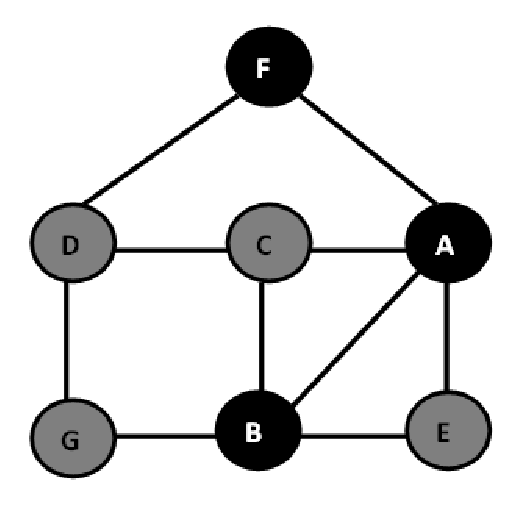
\includegraphics[width=0.5\linewidth]{Figures/cacds5.eps}}
    \label{subfig2}\\
  \caption{(a) CDS Construction with Contention, (b) CDS Construction without Contention}
  \label{aa} 
\end{figure}
Here one can easily see the following CDSs: 
 $$CDS = \{A,B,C\}, \{A,B,F\}, \{C,D,B\}, \{A,B,G\}, \{A,B,C,D\}$$
Among the above CDSs minimum size CDS  are as follows: 
$$MCDS = \{A,B,C\}, \{A,B,F\}, \{C,D,B\}, \{A,B,G\}$$
However the contention aware CDSs are only the followings:
$$CACDS = \{A,B,F\}, \{C,D,B\}, \{A,B,G\}$$
 
 In Fig \ref{aa}(a), if the CDS is constructed in traditional way, node A, B and C can be selected which will lead to contention problem. Because, upon receiving message from node A, if two of its neighbors node B and node C start to \emph{rebroadcast} it, they have to contend with each other first for gaining access to the shared channel as they are within the transmission range of each other. So, the selection of the nodes should be done intelligently to minimize this type of contentions. Figure \ref{aa}(b) presents a scenario, where node F is selected instead of node C to avoid the contention. The new heuristic designed for minimizing contention will never select {A,B,C} in order to avoid contention.

\section{Related Works}
\label{literature}

Researchers have proposed several approaches to reduce the \textit{broadcast storm problem}. A conventional solution to mitigate this problem is to construct a virtual backbone as the basis of routing and broadcasting. The idea to create a virtual backbone using connected dominating set (CDS) is first proposed by Ephermides in \cite{ephremides1987design}. Since then, various methods on the CDS construction have been found in the literature which can be classified as centralized algorithms %\cite{guha1998approximation} 
and distributed algorithms %\cite{lim2001flooding, peng2000reduction}
based on the network information they used.

Multicasting to all nodes in an ad-hoc network is equivalent to broadcast. The problem of constructing optimal broadcast tree that minimizes the number of packet forwarding is very much similar to MCDS problem \cite{lichtenstein1982planar}. MCDS problem cannot be solved in polynomial time, so the optimal broadcast tree construction based on MCDS is proved to be an NP-complete problem. So, researchers have proposed several approximation algorithms and heuristics to find the optimal broadcast tree using the concept of MCDS. 
 
Guha and Khullar first propose two greedy heuristic algorithms in \cite{guha1998approximation}, to construct CDS based on Minimum Connected Dominating Set (MCDS) and Weakly connected dominating set (WCDS). %By using a potential function, Ruan et al. proposed a one-step greedy approximation algorithm \cite{ruan2004greedy} to construct CDS.
In \cite{cheng2004approximation}, authors propose a greedy algorithm for MCDS in unit-disk graphs based on MIS (Maximal Independent Set). Min et al. propose to use a Steiner tree with minimum number of Steiner nodes (ST-MSN) in \cite{min2006improving}.

Due to the lack of global topology information, the distributed approach is most widely used for CDS construction in wireless multi-hop network. Das and Bharghavan in \cite{das1997routing} provide the distributed implementation of the two centralized algorithms given by Guha and Khuller in \cite{guha1998approximation}. Both implementations suffer from high message complexities. The one given by Wu and Li in \cite {wu1999calculating} has no performance analysis. It needs at least two-hop neighborhood information. Lim and Kim ~\cite{lim2001flooding} propose a reactive algorithm called Self Pruning (SP) that uses direct neighborhood information to decide whether to forward a packet or not and another proactive algorithm named Dominant Pruning (DP) where extended neighborhood information is used. In DP, a node construct its own forwarding list from the subset of its 1-hop neighbors in order to cover all its 2-hop neighbors. They also propose two extensions of DP known as Partial Dominant Pruning (PDP) and Total Dominant Pruning (TDP).

Though there are several methods to construct CDS to reduce redundancy but CDS has never been computed to reduce contention in any of the prior works. Therefore, we are proposing to fill up this notable gap by introducing contention aware minimum connected dominating set in this paper.


 
\section{Preliminaries}
\label{Preliminaries}

We use a simple graph $G(V,E)$ to represent an ad-hoc network, where $V$ represents the set of wireless mobile nodes and $E$ represents the set of edges. An edge $(u,v)$ indicates that both hosts $u$ and $v$ are within their transmission range. $N(u)$ is defined as a set of adjacent nodes of node $u$ and $N(N(u))$ is the set of nodes that is at most 2-hop away from node $u$. $F\textsubscript{u}$ represents the list of 1-hop neighbors of $u$ that are selected for forwarding by node $u$. $B\textsubscript{u}$ is the set of 1-hop neighbors of node $u$ that are eligible to be included in the forwarding list $F\textsubscript{u}$. $U\textsubscript{u}$ is the set of nodes that need to be covered by using nodes from $B\textsubscript{u}$ while $u$ creates its forwarding list $F\textsubscript{u}$ . 

MCDS \cite{guha1998approximation} and Dominant Pruning \cite{lim2001flooding} has been used as state-of-art algorithms to evaluate the new proposed approaches. 

\textbf{(i) MCDS Construction Algorithm:} At the start of the algorithm, all nodes in the network are colored white. The node with maximum cardinality is then selected and colored black. All the one-hop neighbors of that node are colored gray. A gray node having maximum number of white neighbors is then selected and colored black. The selection process recursively runs until no white node exits. The set with all the black nodes are the resultant nodes that makes MCDS. In figure \ref{aa}(a), $$MCDS = \{A,B,C\}$$.
 
\textbf{(ii) Dominant Pruning:} The forwarding list creation process of dominant pruning algorithm is as follows:- suppose, a node $v$ receives a packet from node $u$. The sender node $u$ also sends a \textit{forwarding list ($F\textsubscript{u}$)}  with the packet header. If  $v \in F\textsubscript{u}$, then the node $v$ will rebroadcast and will create its own forward list ($F\textsubscript{v}$). The node then start constructing $U\textsubscript{v}$ which is all uncovered two-hop neighbors of $v$. The set $B\textsubscript{v}$ represents those neighbors of $v$ which are possible candidates for inclusion in $F\textsubscript{v}$. Then, in each iteration, $v$ selects a neighbor $w$ $\in$ $B\textsubscript{v}$, such that $w \notin F\textsubscript{v}$ and the list of neighbors of $w$ covers the maximum number of nodes in $U\textsubscript{v}$ , i.e $|N(w)\cap U\textsubscript{v}|$ is maximized. Next $v$ includes $w$ in  $F\textsubscript{v}$ and sets $U\textsubscript{v} =U\textsubscript{v} - N(w)$ . The iterations continue for as long as $U\textsubscript{v}$ becomes empty or no more progress can be accomplished. 
 
\section{Contention aware Connected Dominating Set (CACDS) Construction Algorithm}
A brief description of the proposed algorithms is stated in this section. The first algorithm is a centralized one because it needs the global topology information of a network for constructing CDS and the second one is the distributed algorithm where each node knows only its two hop neighborhood information.   

\begin{figure*}[h]
\begin{minipage}{.25\textwidth}
\centering
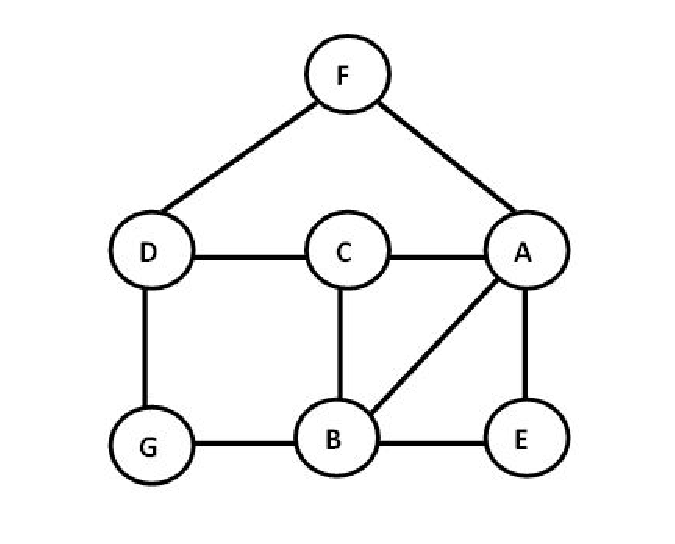
\includegraphics[width=0.9\linewidth,height=.8\linewidth]{Figures/cacds1.eps}
\\(a): All nodes are colored WHITE
\end{minipage}%
\begin{minipage}{.25\textwidth}
\centering
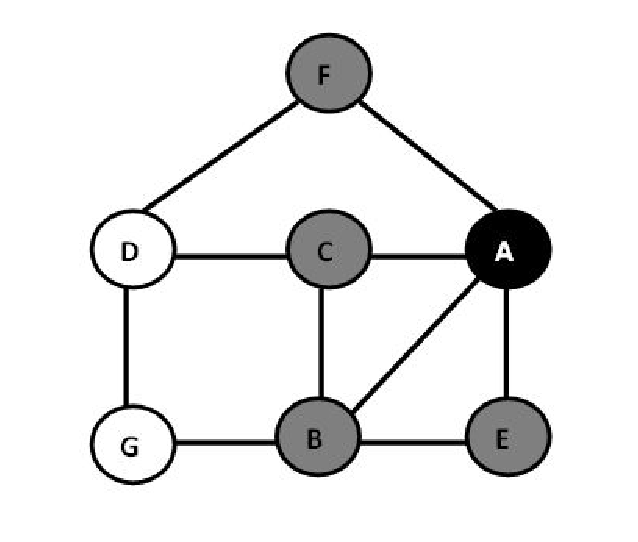
\includegraphics[width=0.9\linewidth,height=.8\linewidth]{Figures/cacds2.eps}
\\(b): Node A is selected and colored BLACK
\end{minipage}%
\begin{minipage}{.25\textwidth}
\centering
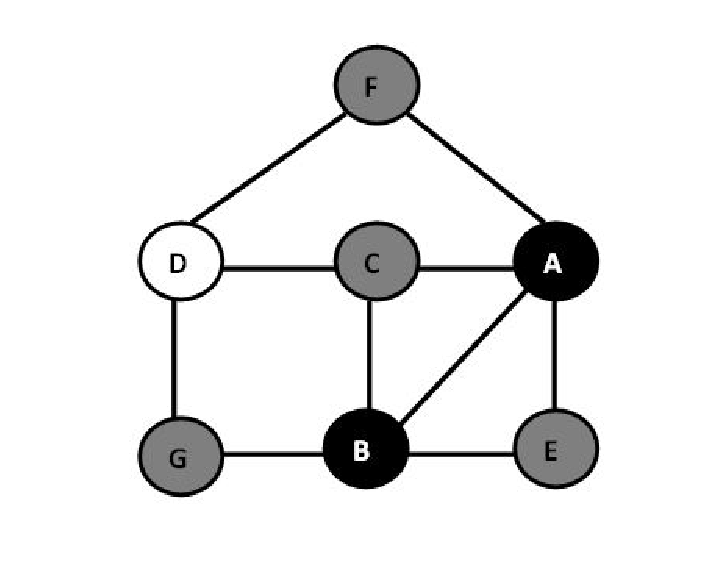
\includegraphics[width=0.9\linewidth,height=.8\linewidth]{Figures/cacds3.eps}
\\(c): Node B is selected and the process continues
\end{minipage}%
\begin{minipage}{.25\textwidth}
\centering
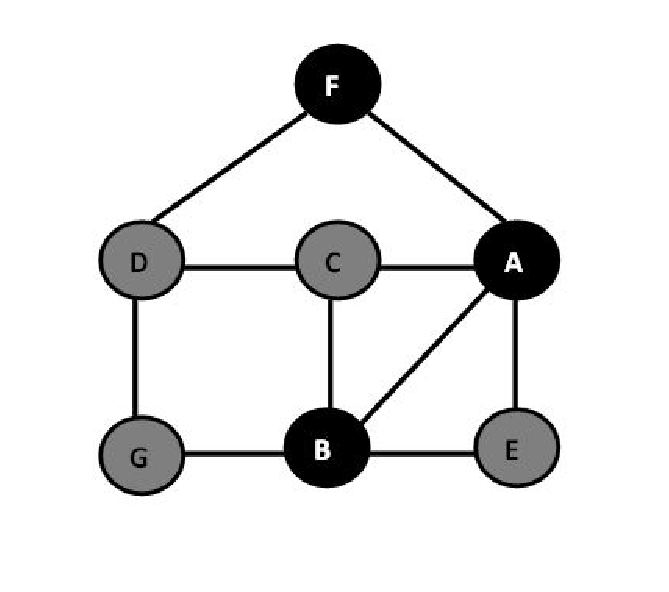
\includegraphics[width=0.9\linewidth,height=.8\linewidth]{Figures/cacds4.eps}
\\(d): Finally node A,B,F constructs the CACDS
\end{minipage}
\caption{ Step by step construction of Centralized Contention aware Connected Dominating Set (Centralized CACDS).}
\label{cds}
\end{figure*}

\subsection{Centralized Contention Aware Connected Dominating Set}
The centralized algorithm is presented in Algorithm \ref{Algorithm1}.
At the start of the algorithm, all the nodes are colored white and placed in $ColorW$ set. That means, $ColorW$ set consists of all nodes $v \in V$. 
%Whenever a node is selected as a forwarding node, the node and all its 1-hop neighbors are discarded from $ColorW$ set. 
The node with the maximum cardinality is then selected from $ColorW$ set and colored as black and placed in a different $ColorB$ set (shown in line 5-6 of Algorithm \ref{Algorithm1}). In case of tie, a node is selected randomly among the ones with maximal cardinality. All the neighbors of that black node are colored as gray and put the in $ColorG$ set. 
%The nodes in $ColorB$ set are the forwarding nodes of the network. When a node $ u \in ColorB$ forwards any message, all of its 1-hop neighbors receive the message and become member of $ColorG$ set. 
Among the gray nodes of $ColorG$ set, the nodes that have minimum number of black neighbors are selected and placed in a set called \textit{$Candidate\_Set$} (shown in line 17-22 of Algorithm \ref{Algorithm1}). The black nodes are already in CDS. Therefore, by selecting a gray node with minimum black neighbors reduces the chance of contention. 
In case of tie,
%Among the nodes in \textit{$Candidate\_Set$} 
the gray node which has maximum number of white neighbors is  selected and colored as black and all its white neighbors are colored as gray (shown in line 23-29 of Algorithm \ref{Algorithm1}) . A recursive selection process runs till there is no white node left in the network. 

The entire selection process is shown using the following example. Consider Figure \ref{cds}, among all the nodes node A has the maximum cardinality (which is 4 here), so, according to the algorithm, node A is colored black and all its neighbors (node B,C,E and F) are colored gray (illustrated in Figure \ref{cds}(b)). In the next step, all the gray nodes have only 1 black neighbor that is node A and each of the gray nodes B, C and F has 1 white neighbor and node E has none. So we can select either of Node B, C , F. Suppose, node B is selected to cover node G and it is colored as black and node G is colored as gray (illustrated in Figure \ref{cds}(c)). The only white node remaining in the network at this stage is node D. The gray node C has now two black neighbors (node A and node B), gray node G and node F each has one black neighbor, so either of node G and node F can be selected. Suppose node F is selected to cover node D ( In Figure \ref{cds}(d)). So, the final Contention aware Connected Dominating Set consists of node A,B and F. So, $$CACDS = \{A,B,F\}$$.
\begin{algorithm}

\caption{Centralized CACDS}
\label{Algorithm1}

\begin{algorithmic}[1]
 \STATE INPUT: G(V,E)
 \STATE RESULT \{CACDS\}
\STATE $ColorB=\emptyset$, $ColorG=\emptyset$, $CACDS=\emptyset$,
\STATE $ColorW$ = all nodes $v\in V$;
\STATE Select a node v $\in$ V with max(degree(v));
\STATE $ ColorB = \{v\} $;
\STATE $ ColorG= N(v)-\{v\}$;
\STATE $ ColorW=ColorW-N(v)$;


\WHILE{$ ColorW \neq \emptyset $}
 
   \STATE $MaxWhite=0$, $MinBlack=\|V\|$, $Candidate\_Set=\emptyset$;
 
        \FORALL{node $u \in ColorG$}
        
            \STATE $BlackCount = \|N(u) \cap ColorB\|$;
            \IF{$ BlackCount < MinBlack $}
                \STATE $MinBlack= BlackCount$;
            \ENDIF
        \ENDFOR
        \FORALL{ node $u \in ColorG$}
        
            \STATE $ BlackCount = \|N(u) \cap ColorB\|$;
            \IF{$BlackCount==MinBlack$}
           \STATE $ Candidate\_Set = Candidate\_Set \cup \{u\} $;
            \ENDIF
        \ENDFOR
            \FORALL{ node $w \in$ $Candidate\_Set$}
                \STATE $ WhiteCount = \|N(w) \cap ColorW\|$;
                \IF{$WhiteCount > MaxWhite$}
                 \STATE  $MaxWhite= WhiteCount$ ;
                 \STATE $selectedNode=w$;
                \ENDIF
            \ENDFOR
            
               
            \IF{$MaxWhite > 0$} 
                \STATE $ ColorB = ColorB \cup \{selectedNode\}; $ 
                \STATE $ColorW = ColorW-N(selectedNode)$; \\
                \STATE $ ColorG = ColorG \cup (N(selectedNode)-ColorB); $
            \ELSE
                \STATE $ColorG = ColorG - Candidate\_Set$;
            \ENDIF
            
\ENDWHILE
\STATE $ CACDS= ColorB$;

\end{algorithmic}
\end{algorithm}


\noindent{\bf Complexity Analysis of Centralized CACDS:}
In the algorithm \ref{Algorithm1}, the iteration of the $While Loop$ (line 9-37 of Algorithm \ref{Algorithm1}) continues until $ColorW$ set does not become empty. At first set $ColorW$ consists of all nodes in the network. So, the loop body will run in $O(V)$ times where $V$ is the total number of nodes in the network. Inside the $While Loop$, there are loops that are used to find the nodes which have minimum number of black neighbors and maximum number of white neighbors each of which individually runs in $O(V)$ times in the worst case scenario. So, the run time complexity of the Centralized CACDS is $O({V}^2)$.

\noindent{\bf Theoretical Correctness of CACDS:}
Next, we show the theoretical correctness of CACDS in the following two lemmas.

\textit{Lemma 1:} $CACDS$ is a connected dominating set.\\
\textit{Proof:} 
%Let us use contradiction to prove that $CACDS$ is a connected dominating set.
The proof is by contradiction.
Suppose the vertex set of CACDS is, $$V_{CACDS} = \{v_1,v_2,v_3...v_m\}$$
Assume node $v\textsubscript{i} \in V_{CACDS}$ cannot communicate with other nodes in $CACDS$. %and $cacds$ is the number of nodes in the $CACDS$.  
According to the algorithm, the black nodes are selected among the gray nodes. When a node becomes gray, that means it has at least one black neighbor in the network. As $v_i$ is a member of $CACDS$, the node must be black. When $v_i$ was selected, it was among one of the gray nodes and each gray node is connected to one of the black nodes. Therefore, each black node has at least one path to communicate with other nodes in $CACDS$. The result contradicts with the hypothetic premises. So, $v_i$ must have a path to connect other nodes in the $CACDS$. Hence each node in $CACDS$ must be connected. 

\textit{Lemma 2:} The connected dominating set constructed by $CACDS$ covers all the nodes in the network.\\
\textit{Proof:} Assume that, $U$ is the set consisting of all the nodes in the network, $U = \{x\textsubscript{1},x\textsubscript{2},...x\textsubscript{n}\}$, $n$ is the number of nodes in the network, and vertex set of CACDS is $V_{CACDS} = \{v_1,v_2,v_3...v_m\}$,
%$CACDS = \{v\textsubscript{1},v\textsubscript{2},v\textsubscript{3}...v\textsubscript{cacds}\}$
where $m$ is the total number of nodes in the $CACDS$. $N(v\textsubscript{i})$ is the set of nodes which become gray after selecting $v\textsubscript{i}$ as a member of $CACDS$ i.e., $N(v\textsubscript{i})$ represents the set consisting of all adjacent nodes of $v\textsubscript{i}$.\\
\begin{equation}
N = N(v\textsubscript{1}) \cup N(v\textsubscript{2}) \cup N(v\textsubscript{3}) \cup ... N(v\textsubscript{m})
\end{equation}
In order to prove, $CACDS$ covers all the nodes in the network, we have to prove that $U = N$.
As $CACDS$ is a connected dominating set, so every node $x\textsubscript{i} \in U$  either same as $v\textsubscript{j}$ or is adjacent to $v\textsubscript{j}$ for some $j$. In other words the following proposition must hold, 
$$ \forall i \Big[\exists j \big[x_i \in N(v_j) \big] \Big]$$
%Let $x\textsubscript{1} \in N(v\textsubscript{1})$;  $x\textsubscript{2} \in N(v\textsubscript{2})$; $x\textsubscript{n} \in N(v\textsubscript{m})$  
Thus,

\begin{equation}
    \{x\textsubscript{1},x\textsubscript{2},...x\textsubscript{n}\} \subseteq N(v\textsubscript{1}) \cup N(v\textsubscript{2}) \cup N(v\textsubscript{3}) \cup ... N(v\textsubscript{m}) 
    \label{eqn1}
\end{equation} 
From Equation \ref{eqn1},
\begin{equation}
   \{x\textsubscript{1},x\textsubscript{2},...x\textsubscript{n}\} \subseteq N
   \label{eqn2}
\end{equation}
By definition,
\begin{equation}
    \{x\textsubscript{1},x\textsubscript{2},...x\textsubscript{n}\} \subseteq U
    \label{eqn3}
    \end{equation}
 From Equation \ref{eqn2} and \ref{eqn3}, by the axiom of extensionality, we can say that, \\  
    \begin{equation}
\forall x_i (x_i \in U \Longleftrightarrow x_i \in N) \implies U = N
 \end{equation}

\subsection {Distributed Contention aware Connected Dominating Set (Distributed CACDS)}

For distributed CACDS, it is assumed that, each node knows its 2-hop neighborhood information. After receiving a packet from node $u$, if node $v$ finds itself in node $u$'s \textit{forward list}, it starts to make its own \textit{forward list} ($F\textsubscript{v}$) from a subset of its one-hop neighbors ($B\textsubscript{v}$) to cover all of its uncovered two-hop neighbors ($U\textsubscript{v}$). The sets $U_v$ and $B_v$ is calculated using the following equations:
% \begin{equation}
$$U\textsubscript{v} = N(N(v)) - N(v) - N(u)$$
%\end{equation}
%\begin{equation}
$$B\textsubscript{v} = N (v)- N (u) $$
%\end{equation}

 \begin{figure*}[h]
\begin{minipage}{.33\textwidth}
\centering
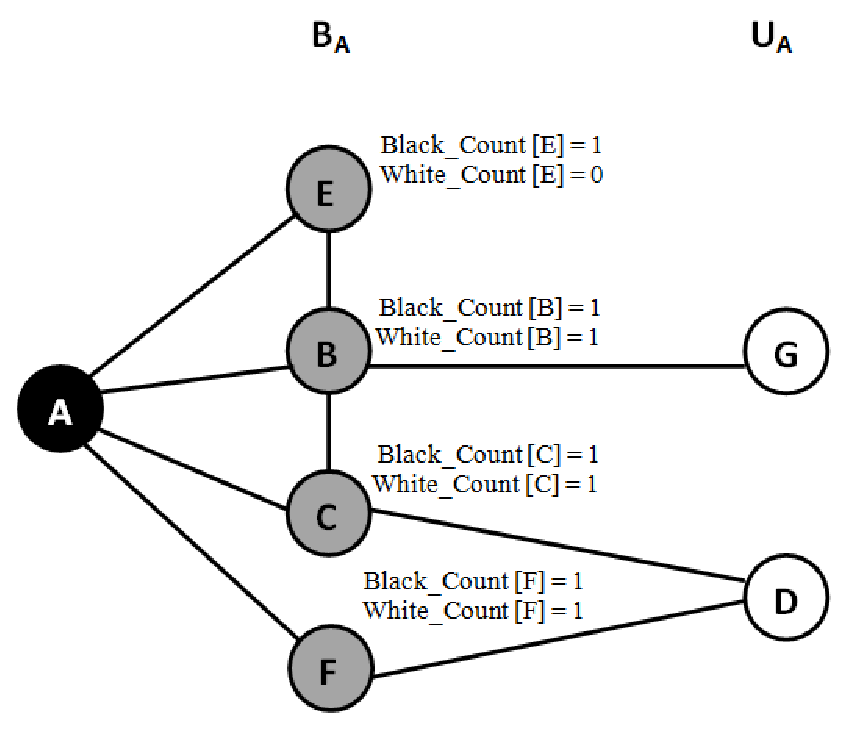
\includegraphics[width=0.8\linewidth,height=.7\linewidth]{Figures/dis1.eps}%
\\(a): Connection of node A with B\textsubscript{A} and U\textsubscript{A}
\end{minipage}%
\begin{minipage}{.33\textwidth}
\centering
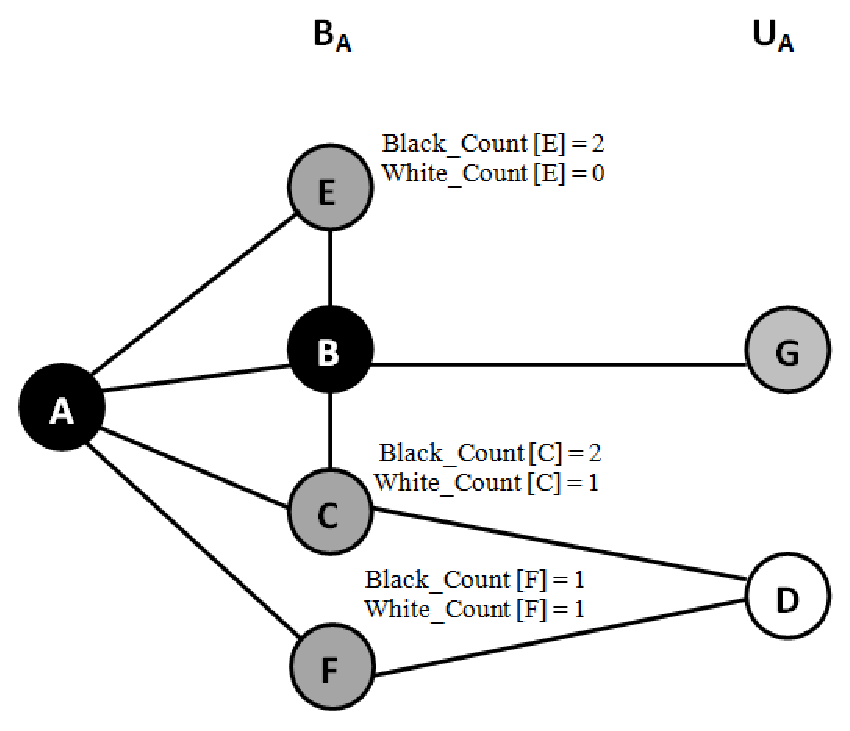
\includegraphics[width=0.8\linewidth,height=.7\linewidth]{Figures/dis2.eps}
\\(b): Node B is selected for F\textsubscript{A}
\end{minipage}
\begin{minipage}{.33\textwidth}
\centering
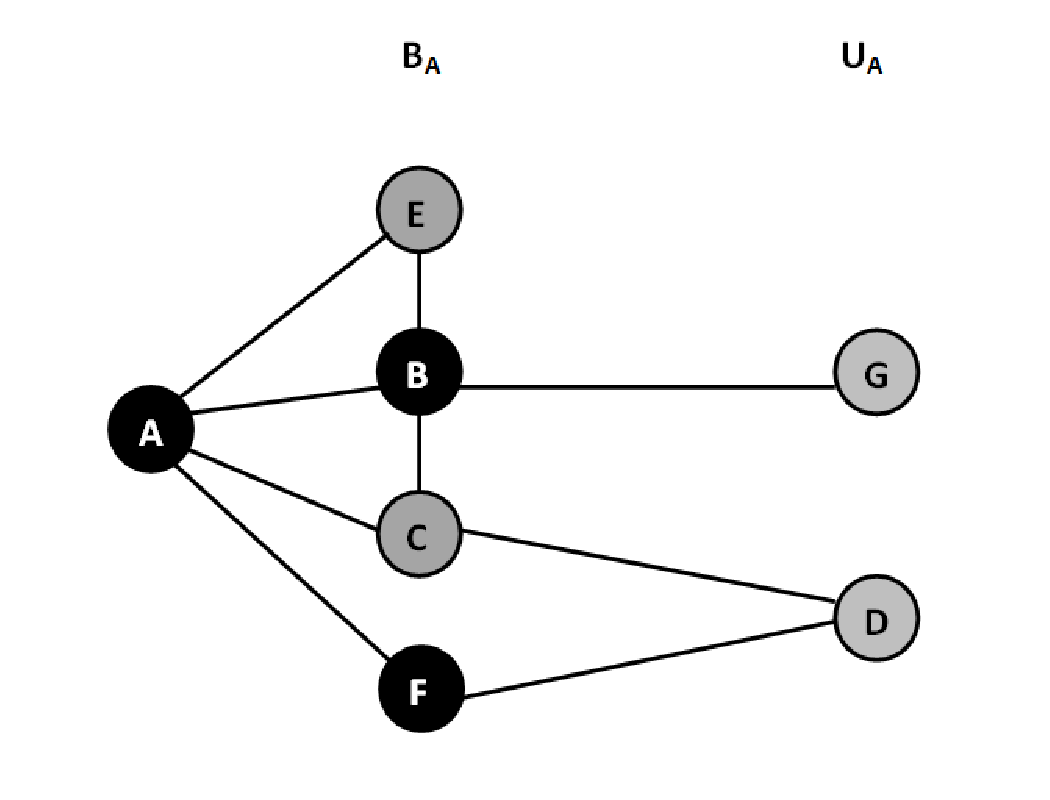
\includegraphics[width=0.8\linewidth,height=.7\linewidth]{Figures/dis3.eps}
\\(c): Node F finally selected for F\textsubscript{A}
\end{minipage}
\caption{ Step by step construction of Forward\_list of node A }
\label{dis}
\end{figure*}

 The new approach is stated in Algorithm 2. In the algorithm, an array named $Black\_Count$ is used so that each node  $p \in B\textsubscript{v}$ can keep track of its adjacent nodes in $B\textsubscript{v}$  that are already selected in the \textit{forwarding list}. At the start of constructing $F\textsubscript{v}$,  the corresponding value in the $Black\_Count$ array of all the nodes $p \in B\textsubscript{v}$ is set to one. The nodes whose corresponding value of the $Black\_Count$ is minimum among all the nodes in $B\textsubscript{v}$ are placed into a $Candidate\_Set$ (shown in line 13-17 of Algorithm \ref{Algorithm2}). Then in each iteration, a node $x \in Candidate\_Set$ is selected which covers maximum number of nodes in $U\textsubscript{v}$, i.e., $\|N(x) \cap U\textsubscript{v}\|$ is maximized (shown in line 18-30 of Algorithm \ref{Algorithm2}). Next, node $v$ includes node $x$ in its forwarding list $F\textsubscript{v}$ and the corresponding values of the $Black\_Count$ of the nodes in $B\textsubscript{v}$ adjacent to $x$ are all increased by one (shown in line 32-36 of Algorithm \ref{Algorithm2}). Node $v$ then updates $U\textsubscript{v} = U\textsubscript{v} - N(x)$  and $B\textsubscript{v} = B\textsubscript{v} - x$. This process is iterated until all nodes in $U_v$ is covered or no change in $B_v$ set is possible.

Let us explain the process using an example scenario. Consider Figure \ref{cds}. Suppose node A is the broadcast initiator. Figure \ref{dis} is the redrawing of Figure \ref{cds} for better visualization in order to determine the \textit{forward\_list} of node A. $B\textsubscript{A}$ consists of node B, C, E and F and $U\textsubscript{A}$ consists of node D and G. In DP, node A selects node B and C for forwarding the message to cover node G and D. This selection arises contention between node B and node C when they start to rebroadcast.

The proposed algorithm aims at minimizing this type of contention. The algorithm does not select node C to cover node D if node A decides to choose node B to cover node G. It selects node F instead to cover node D to avoid contention. So, node B and F will be in the forward list of node A. Hence, $F\textsubscript{A}=\{B,F\}$. The whole process is shown in Table \ref{table:5}.
\begin{algorithm}
\caption{Creation of forward\_list of a node $v$}

\label{Algorithm2}
\begin{algorithmic}[1]
\STATE $Forwarding\_node \leftarrow v$
\STATE $F\textsubscript{v} = \emptyset$, $size\_of\_forward\_list=0$,

 \FORALL{node $p \in B\textsubscript{v}$}
    \STATE $Black\_Count[p] = 1$;
 \ENDFOR
\WHILE{$ U\textsubscript{v} \neq \emptyset $ or $B_v$ remains unchanged}
    \STATE $maximum = 0$, $minimum=\|V\|$, $Candidate\_Set=\emptyset$;
    
    \FORALL{node $q \in B\textsubscript{v}$}
        \IF{$Black\_Count[q] < minimum$}
            \STATE $minimum = Black\_Count[q] $;
        \ENDIF
    \ENDFOR
     \FORALL{node $r \in B\textsubscript{v}$}
        \IF{$ Black\_Count[r] == minimum $}
            \STATE $Candidate\_Set = Candidate\_Set \cup \{r\}$;
        \ENDIF
     \ENDFOR
     
     \FORALL{node $s \in Candidate\_Set$}
        \FORALL{node $t \in U\textsubscript{v}$}
            \IF{node $t \in N(s)$}
                \STATE $ White\_Count[s] = White\_Count[s]+1 $;
            \ENDIF
        \ENDFOR
    \ENDFOR
    
     \FORALL{node $i \in Candidate\_Set$}
        \IF{$White\_Count[i] > maximum$}
            \STATE $maximum = White\_Count[i]$;
            \STATE $x = i$;
        \ENDIF
    \ENDFOR
     \IF{$maximum > 0$}   
     \STATE $F\textsubscript{v}[size\_of\_forward\_ list] = \{x\}$;
     \STATE $size\_of\_forward\_ list = size\_of\_forward\_ list + 1$;
     \FORALL{node $y \in (B\textsubscript{v} \cap N(x))$}
        \STATE $ Black\_Count[y]= Black\_Count[y]+1$;
    \ENDFOR
     \STATE $ U\textsubscript{v} = U\textsubscript{v} - N(x)$;
      \STATE $B\textsubscript{v} = B\textsubscript{v}-\{x\}$;
     \ENDIF
\ENDWHILE
\end{algorithmic}
\end{algorithm}
\begin{table}[h]

  \begin{center}
    \caption{Forwarding lists creation process in Distributed CACDS algorithm for the scenario of Figure \ref{cds}(a) (node A is the source of broadcast)}.
     \medskip
    \label{table:5}
    \renewcommand{\arraystretch}{1}
       \begin{tabular} {|>{\centering\arraybackslash}p{1cm}|>{\centering\arraybackslash}p{1cm} |>{\centering\arraybackslash}p{1.5cm} | >{\centering\arraybackslash}p{2cm}|>{\centering\arraybackslash}p{1cm}|}
      \hline
      \bf{Previous node ($u$)} & \bf{Current node ($v$)} & \bf{$U\textsubscript{v}$} & \bf{$B\textsubscript{v}$} & \bf{$F\textsubscript{v}$} \\
      \hline
      $\emptyset$ & A &\{B,C,E,F\} &\{G,D\} &\{B,F\} \\
      \hline
      A  & B  & \{G\}& \{D\} & \{G\}  \\
      \hline
      A  & F  & \{D\} & \{G\} & \{D\}  \\
      \hline
      B  & G & \{D\} & \{F\} & \{D\} \\
      \hline
      F  & D &\{C,G\}& \{B\} & \{C\}    \\
      \hline
      D  & C & \{A,B\} & \{E\}& \{A\}   \\
      \hline
    
    \end{tabular}

  \end{center}
\end{table}

\noindent{\bf Complexity Analysis of Distributed CACDS:}
Constructing the $forwarding\_list$ of a node $v$ is very much similar to set cover problem.  Suppose, the maximum degree of a node is $\Delta$. In the worst case scenario the size of $B\textsubscript{v}$ set of a node v can be equal to $\Delta$, i.e. $|B\textsubscript{v}| = \Delta$. Forwarding nodes should be chosen from the set $B\textsubscript{v}$ to cover the nodes that belong to set $U\textsubscript{v}$. The maximum number of nodes in $U\textsubscript{v}$ set that can be covered by $B\textsubscript{v}$ is $\Delta^2$. So, final run time of constructing the $forwarding\_list$ of node $v$ is $O(\Delta^3)$.

 
\section{Experimental Results}
\label{Experimental Results}

\subsection{Simulation Environment}
\begin{figure}[h] 
    \centering
  \subfloat[]{%
       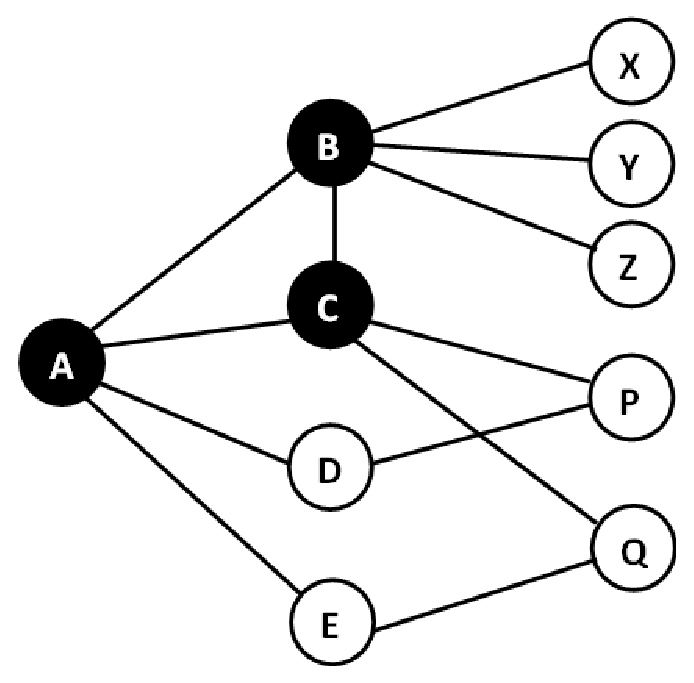
\includegraphics[width=0.45\linewidth, height=35mm]{Figures/forwarding1.eps}}
    \label{subfig1}\hfill
  \subfloat[]{%
        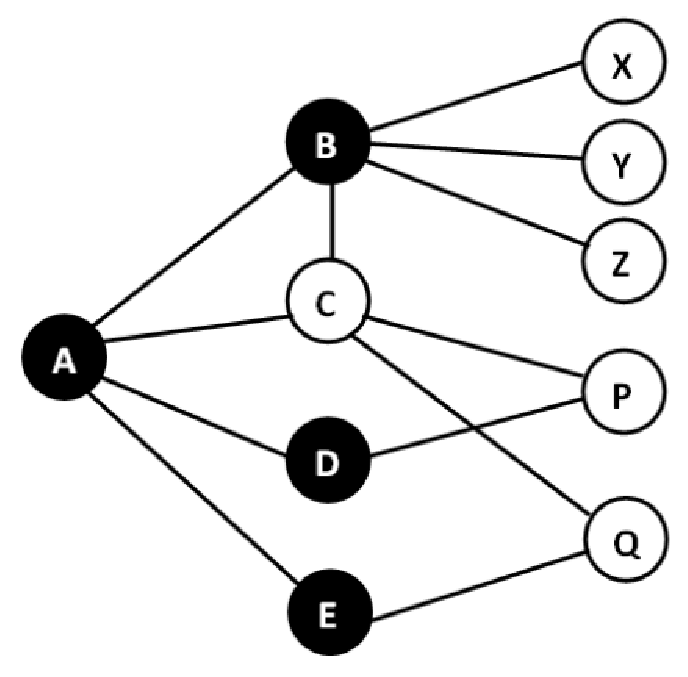
\includegraphics[width=0.45\linewidth, height = 35mm]{Figures/forwarding2.eps}}
    \label{subfig2}\\
  \caption{(a) CDS to minimize redundancy, (b) CACDS to minimize contention}
  \label{ac} 
\end{figure}
To evaluate the performance, randomly deployed networks of 100-500 nodes over a fixed 625m X 625m square region has been simulated. The transmission radius is limited between 125m to 225m. 
%Each node is placed randomly in the simulation space for testing purpose. 
For each scenario 10 different networks are generated and the mean value of the number of forwarding nodes and the amount of contention are taken to evaluate the effectiveness of the proposed algorithms. The simulation code-base is built using C++ programming language. 

\subsection{Performance Metrics}
While evaluating the algorithms, the number of forwarding nodes and the number of contention have been chosen as performance metrics.
%\begin{enumerate}

 \textbf{ (i) Number of forwarding nodes:} The total number of forwarding nodes needed to complete a broadcast is same  as the size of a CDS. Thus we calculate the size of the constructed CDS to determine number of forwarding. In order to minimize contention, the nodes that can reach the maximum number of nodes in the network may to get selected. Therefore, the number of forwarding nodes might increase in order to mitigate contention.  Such a scenario is depicted in Figure \ref{ac}. The number of forwarding nodes is 3 in traditional MCDS algorithm. The number of forwarding nodes increases to 4 in order to minimize contention.

  \textbf{ (ii) Number of Contention:} The total number of contention to complete a broadcast is determined as follows. At first we define ``per hop contention'' which is the number of nodes in the forwarding list of any node $v$ that are neighbors of each other. If one of the members of the $F\textsubscript{v}$ is connected (within the transmission range) to another ones, then those nodes face contentions when they try to forward the packet. Thus per hop contention  ($\mathcal{P}$) is mathematically determined as:  
  $$  \mathcal{P}(v) = \sum_{w \in F\textsubscript{v}} \Big(\big|(N(w)-\{w\}) \cap F\textsubscript{v}\big|\Big)/2$$
Suppose, to complete a broadcast the nodes in $\mathcal{S} = \{v_1,v_2,v_3, ... , v_{cacds}\}$ forward the packet, i.e., $\mathcal{S}$ is the CDS. Let $\mathcal{F}$ represents the set of all the forwarding list that are created at each hop. $$\mathcal{F} =  \{F_{v_1},F_{v_2},F_{v_3},....,F_{v_{cacds}} \}$$
 When we sum up per hop contention of all the forwarding nodes in the network, we get the total number of contention $\mathcal{N}$ that would occur for a broadcast which is mathematically defined as: 
$$  \mathcal{N} = \sum_{v_i \in \mathcal{S}} \mathcal{P}(v_i)= \sum_{v_i \in \mathcal{S}} \sum_{w \in \mathcal{F}_{v_i}}\Big(\big|(N(w)-\{w\}) \cap \mathcal{F}_{v_i}\big|\Big)/2 $$

%\end{enumerate}
\subsection{Experimental Results regarding Number of Forwarding}
For better readability of the results, we have separated the graphs of centralized (MCDS and Centralized CACDS) and distributed (DP and distributed CACDS) algorithms. In Figure \ref{outf100c} and \ref{outf100d}, the effect of centralized and distributed algorithms is presented. The number of node has been set to 100. The size of Centralized CACDS and MCDS is almost same for this scenario. In distributed environment, proposed algorithm needs 1-5\% additional transmissions which is not very high. 
 \begin{figure}[h]
    \centering
    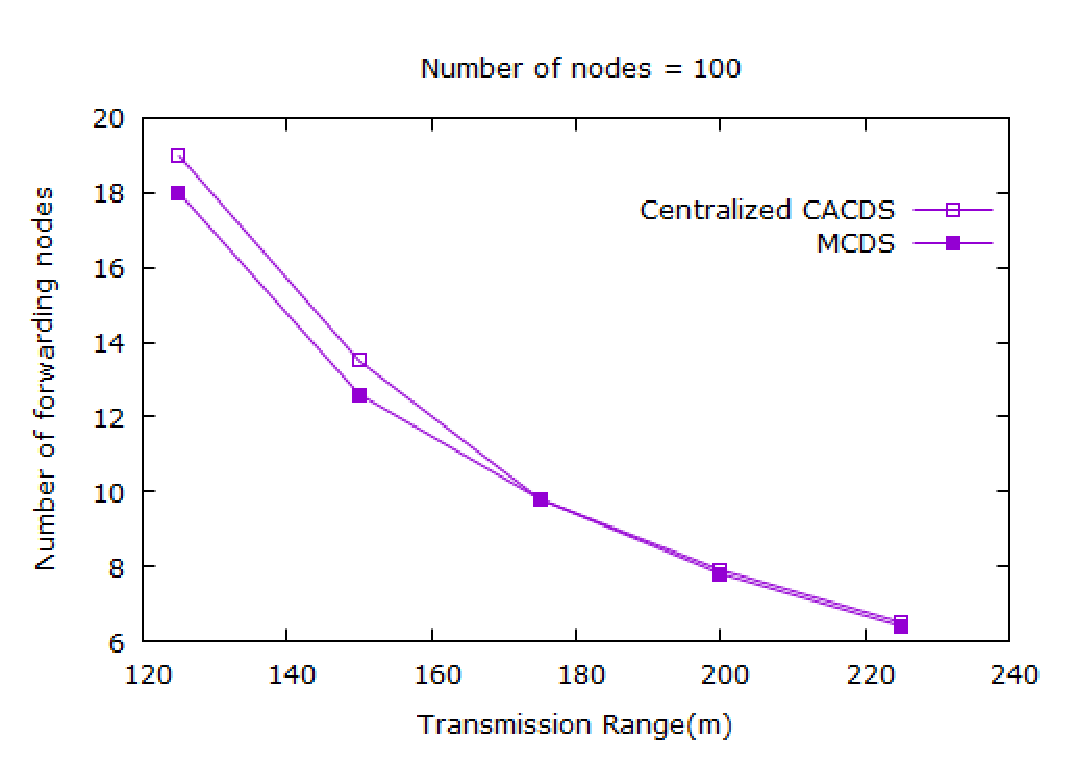
\includegraphics[width=90mm, height=57mm]{Figures/outf100c.eps}
    \caption{Performance of Centralized Algorithms for number of required transmissions of networks having 100 nodes by varying transmission range}
    \label{outf100c}
    \end{figure}
    
    \begin{figure}[h]
    \centering
    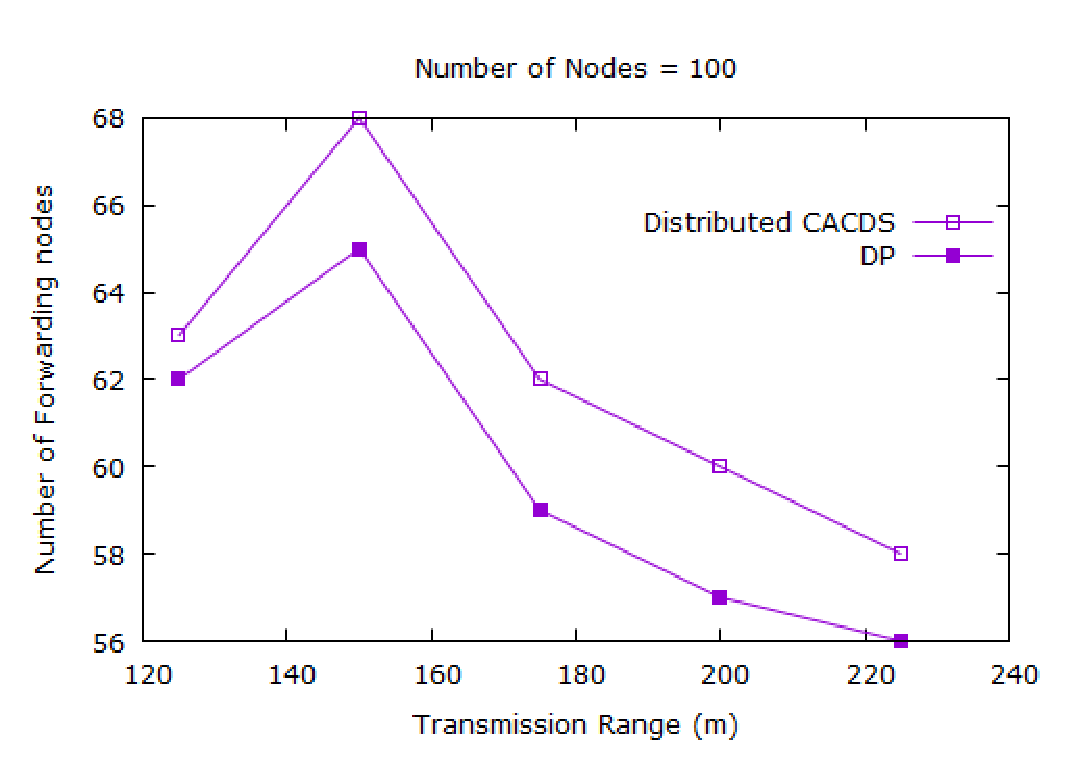
\includegraphics[width=90mm, height=57mm]{Figures/outf100d.eps}
    \caption{Performance of Distributed Algorithms for number of required transmissions of networks having 100 nodes by varying transmission range}
    \label{outf100d}
\end{figure}

Figure \ref{outf225c} and \ref{outf225d} shows the required transmissions by adding nodes in a fixed transmission range (225m). Here also the difference in number of forwarding nodes is very small for both centralized and distributed cases. 
\begin{figure}[h]
    \centering
    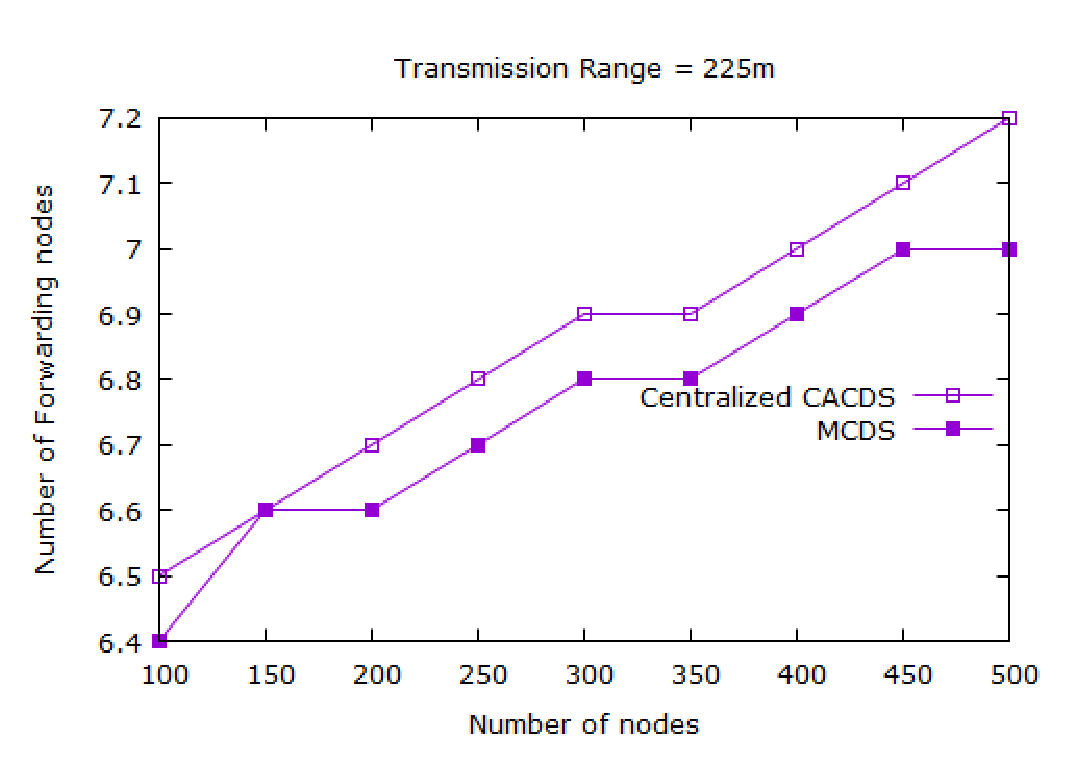
\includegraphics[width=90mm, height=57mm]{Figures/outf225c.eps}
    \caption{Performance of Centralized Algorithms for number of required transmissions by varying number of nodes}
    \label{outf225c}
    \end{figure}
    \begin{figure}[h]
    \centering
    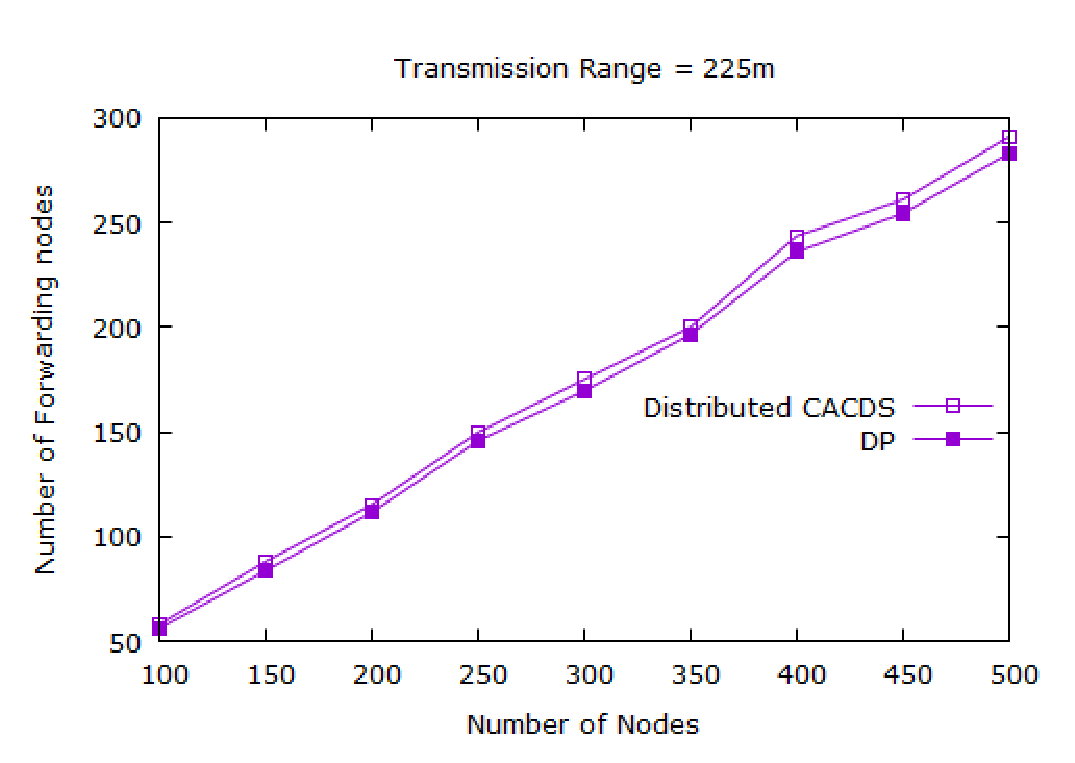
\includegraphics[width=90mm, height=57mm]{Figures/outf225d.eps}
    \caption{Performance of Distributed Algorithms for number of required transmissions by varying number of nodes}
    \label{outf225d}
\end{figure}

\subsection{Experimental Results regarding the Number of Contention}
\begin{figure}[h]
    \centering
    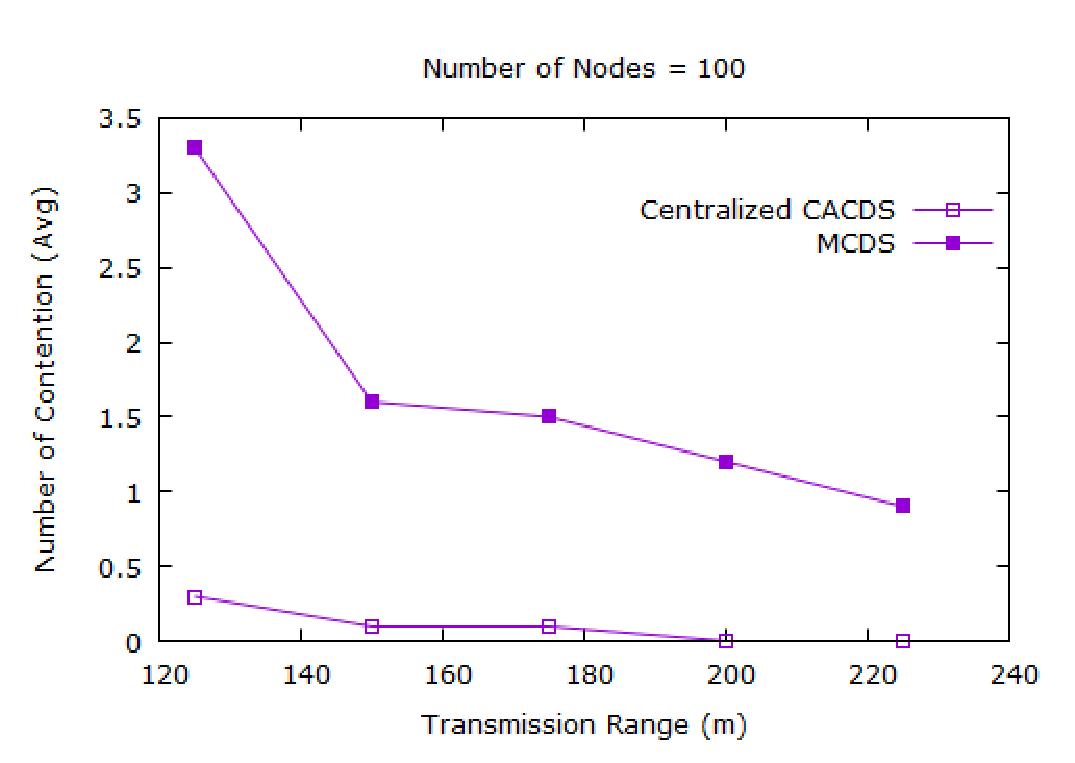
\includegraphics[width=90mm, height=57mm]{Figures/outc100c.eps}
    \caption{Performance comparison of Centralized Algorithms in term of contention varying transmission range}
    \label{outc100c}
    \end{figure}
    \begin{figure}[h]
    \centering
    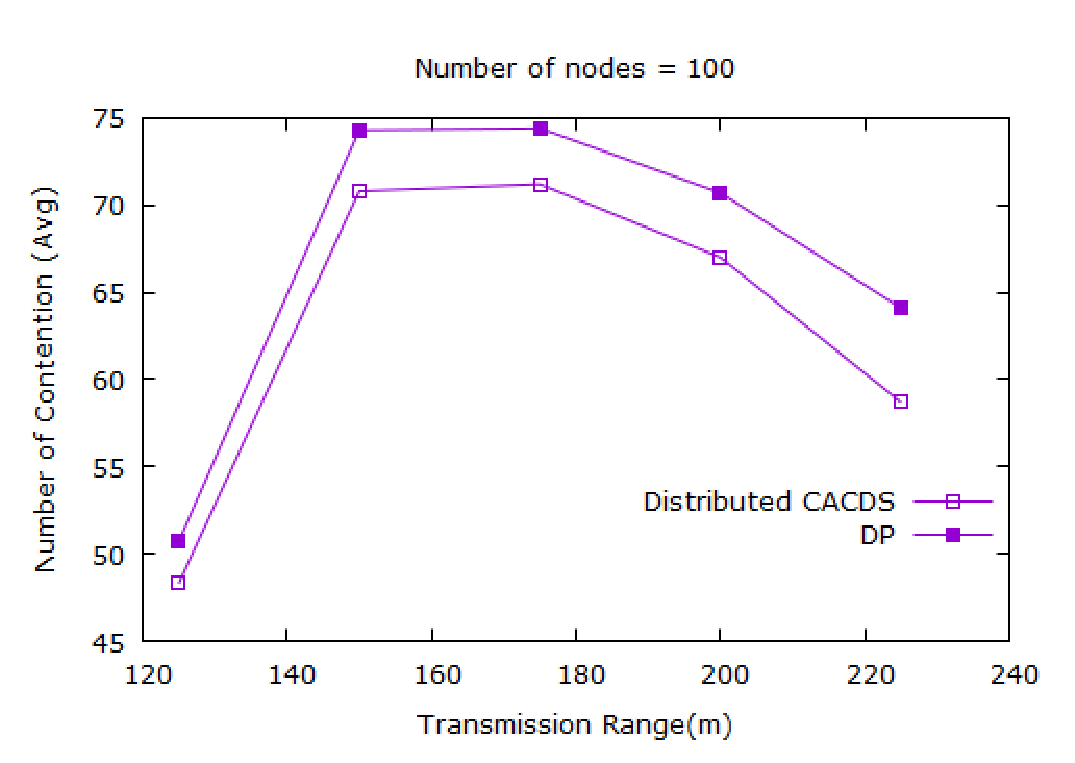
\includegraphics[width=90mm, height=57mm]{Figures/outc100d.eps}
    \caption{Performance comparison of Distributed Algorithms in term of contention varying transmission range}
    \label{outc100d}
\end{figure}

Figure \ref{outc100c} and Figure \ref{outc100d} present the state of contention occurrence for a sparse network with 100 nodes for both the centralized and distributed algorithms respectively. Figure \ref{outc100c} shows that the number of contention varies from 0.9 to 3.3 (in average) between the forwarding nodes in MCDS algorithm whereas it is minimized to 0-0.3 (in average) for Centralized CACDS. It is noticeable that for transmission range 225m, new algorithm generates totally contention free CDS. The distributed scenario is presented in Figure \ref{outc100d}. In distributed environment also, proposed method performs better than that of DP. It  avoids almost 4-9\% contention. In the scenario shown in Figure \ref{outc225c} and Figure \ref{outc225d} we vary number of nodes by keeping the transmission range set to 225m. Needless to say that, the new approaches also perform well.
\begin{figure}[h]
    \centering
    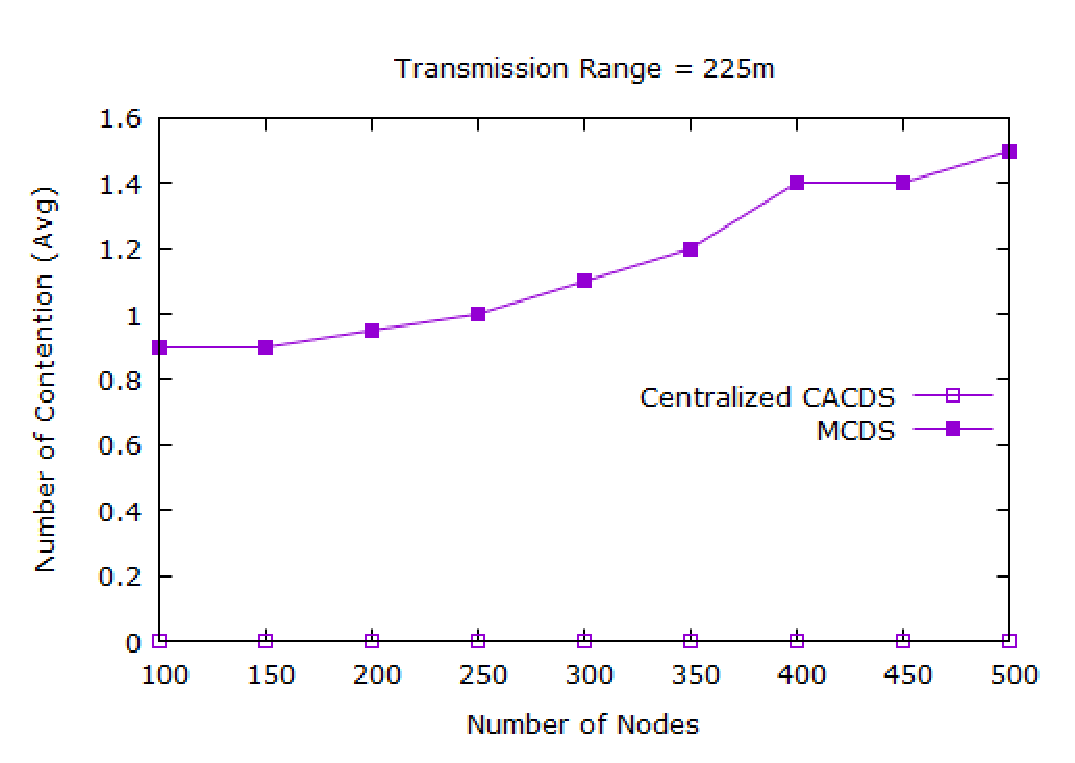
\includegraphics[width=90mm, height=57mm]{Figures/outc225c.eps}
    \caption{Performance comparison of Centralized Algorithms in term of contention varying number of nodes}
    \label{outc225c}
    \end{figure}
    \begin{figure}[h]
    \centering
    \includegraphics[width=90mm, height=57mm]{Figures/outc225d.png}
    \caption{Performance comparison of Distributed Algorithms in term of contention varying number of nodes}
    \label{outc225d}
\end{figure}


\section{Conclusion and Future Work}
\label{conclusion}

In this paper, a new approach has been introduced to construct CDS for minimizing contention. Both centralized and distributed version of the algorithm have been designed and a comprehensive simulation has been presented to analyze the behavior of the proposed algorithms. The simulation result shows that, the proposed algorithm works better in terms of minimizing the contention with a slight increase in the number of forwarding.
The distributed version experience more contentions than centralized version. We are currently experimenting to minimize the performance gap between the two versions. \cite{GOLDBERG200249}
%Because of contention, data sent from one node to another is delayed and it prolongs the execution speed of the network. The execution speed of the network will also increase because of minimizing contention. In the future, analysis of the speed of execution of network will be considered as performance metric to evaluate the proposed algorithms.

\bibliography{bib}
\bibliographystyle{IEEEtran}


\end{document}


